
%(BEGIN_QUESTION)
% Copyright 2015, Tony R. Kuphaldt, released under the Creative Commons Attribution License (v 1.0)
% This means you may do almost anything with this work of mine, so long as you give me proper credit

Calculate the current measured by each ammeter assuming the motor's power consumption is 95 kW, the phase rotation is CBA, and $V_A = 277 \angle -20^o$.  Be sure to express each current value in polar form:

$$\includegraphics[width=15.5cm]{i00849x01.eps}$$

Ammeter ``A'' current = \underbar{\hskip 50pt}

\vskip 10pt

Ammeter ``B'' current = \underbar{\hskip 50pt}

\vskip 10pt

Ammeter ``C'' current = \underbar{\hskip 50pt}

\vskip 10pt

\underbar{file i00849}
%(END_QUESTION)





%(BEGIN_ANSWER)

First, calculating line current magnitude (assuming a balanced 3-phase motor):

$$P = I_{line} V_{line} \sqrt{3}$$

$$I_{line} = {P \over V_{line} \sqrt{3}}$$

$$I_{line} = {95000 \hbox{ W} \over (480 \hbox{ V}) \sqrt{3}}$$

$$I_{line} = 114.27 \hbox{ A}$$

Next, calculating CT secondary current magnitude:

$$I_{CT} = (114.27 \hbox{ A})\left(5 \over 200 \right)$$

$$I_{CT} = 2.857 \hbox{ A}$$

The phase angle of each line current may be determined by the phase rotation.  Given a CBA phase rotation, phase B will be 120 degrees ahead of (leading) phase A, and phase C will be another 120 degrees ahead of (leading) phase B.  Therefore:

\vskip 10pt

Ammeter ``A'' current = \underbar{$2.857$ A $\angle$ $-20^o$}

\vskip 10pt

Ammeter ``B'' current = \underbar{$2.857$ A $\angle$ $100^o$}

\vskip 10pt

Ammeter ``C'' current = \underbar{$2.857$ A $\angle$ $220^o$}

\vskip 10pt

%(END_ANSWER)





%(BEGIN_NOTES)


%INDEX% Electronics review: 3-phase electrical power 
%INDEX% Electronics review: AC motor horsepower calculation (three-phase)

%(END_NOTES)

